\appendix

\section{Benchmark Corpus Details}

\begin{table}[h]
\centering
\caption{Full benchmark corpus with extracted features}
\label{tab:benchmark-corpus}
\begin{tabular}{lllll}
\toprule
Benchmark & Task Type & Modality & Primary Metric & Dataset Size \\
\midrule
ImageNet & Classification & Image & Top-1 Accuracy & 50,000 \\
COCO & Detection & Image & mAP & 5,000 \\
PASCAL VOC & Detection & Image & mAP & 4,952 \\
CelebA & Classification & Image & Accuracy & 19,962 \\
CIFAR-10 & Classification & Image & Accuracy & 10,000 \\
WMT14 & Translation & Text & BLEU & 3,003 \\
WMT16 & Translation & Text & BLEU & 2,999 \\
IWSLT & Translation & Text & BLEU & 1,568 \\
SQuAD & QA & Text & F1/EM & 10,570 \\
Natural Questions & QA & Text & F1 & 7,830 \\
TriviaQA & QA & Text & F1/EM & 11,313 \\
HotpotQA & QA & Text & F1/EM & 7,405 \\
LibriSpeech & ASR & Audio & WER & 2,620 \\
Common Voice & ASR & Audio & WER & 16,164 \\
VGGSound & Classification & Audio & Accuracy & 15,506 \\
VoxCeleb & Verification & Audio & EER & 4,874 \\
MS-COCO (multimodal) & Captioning & Multimodal & BLEU/CIDEr & 5,000 \\
Conceptual Captions & Captioning & Multimodal & CIDEr & 15,840 \\
Visual Genome & Detection & Multimodal & mAP & 5,000 \\
MSCOCO Captions & Captioning & Multimodal & CIDEr & 5,000 \\
\bottomrule
\end{tabular}
\end{table}

\section{Citation Co-Occurrence Matrix}

\begin{figure}[h]
\centering
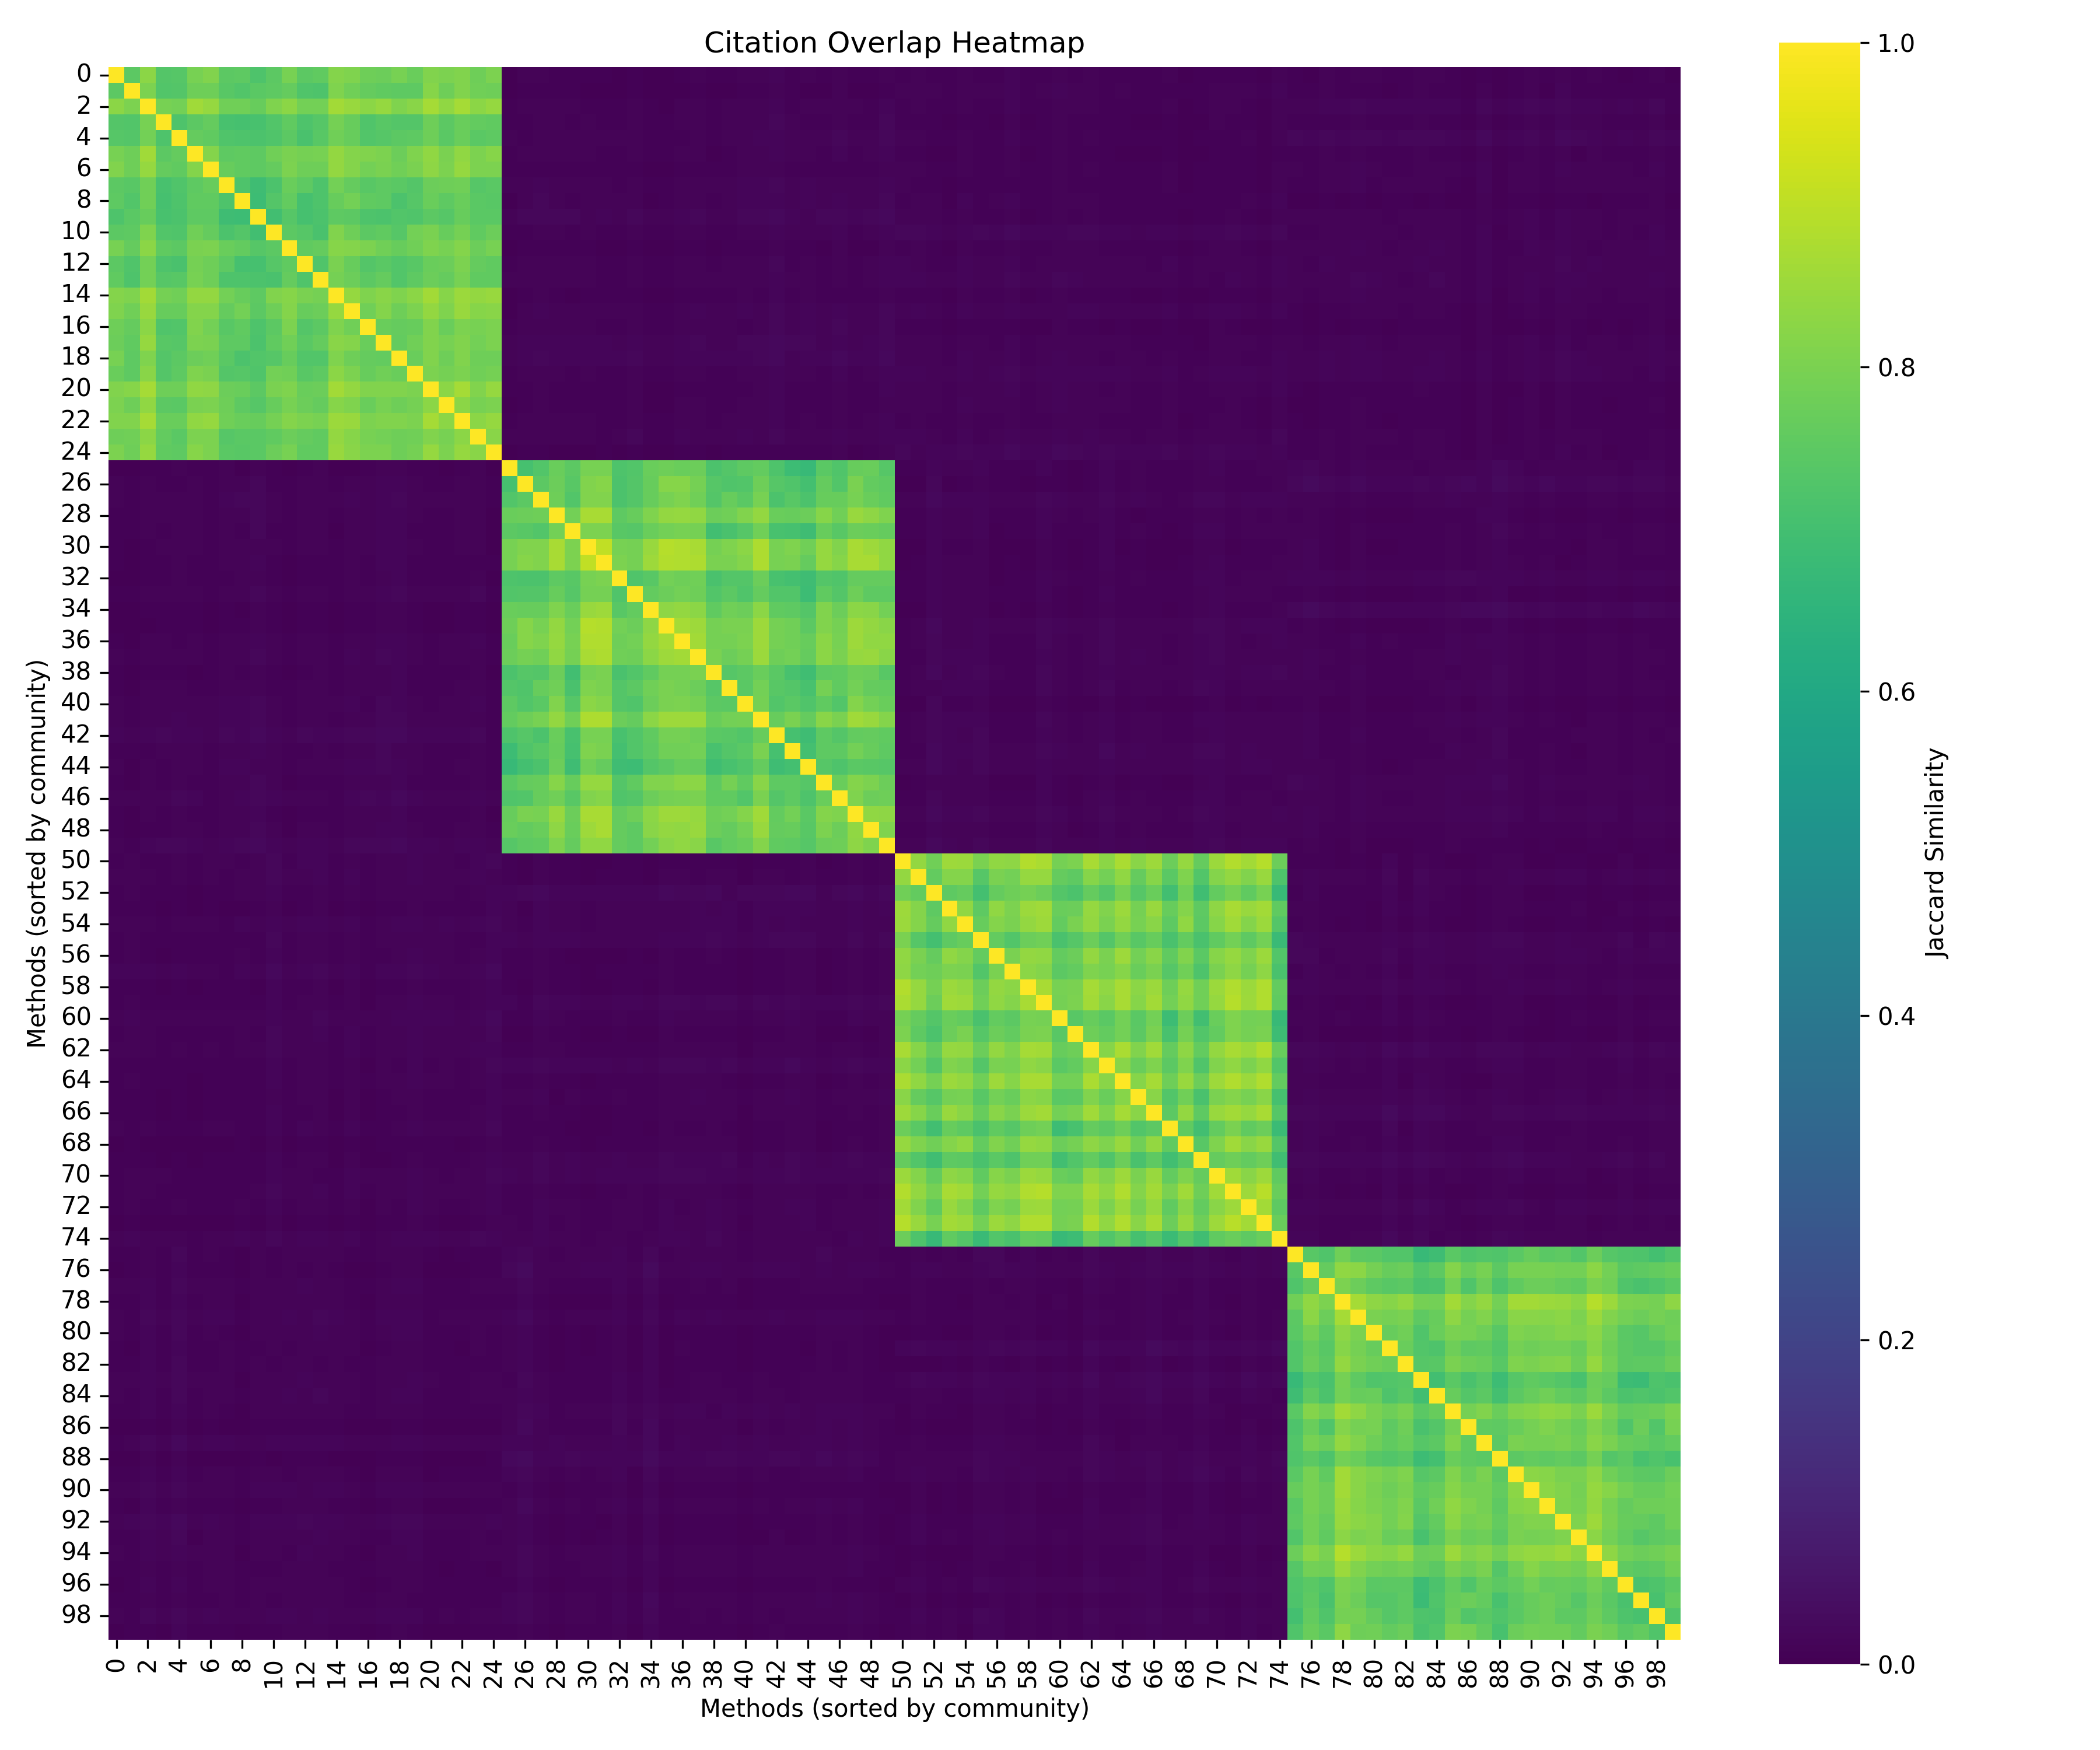
\includegraphics[width=0.8\textwidth]{figures/citation_heatmap.png}
\caption{Pairwise citation co-occurrence (Jaccard similarity) across all benchmarks. Darker cells indicate higher overlap. Clear block-diagonal structure confirms modality-driven families.}
\label{fig:citation-heatmap}
\end{figure}

\section{Embedding Space Visualization}

\begin{figure}[h]
\centering
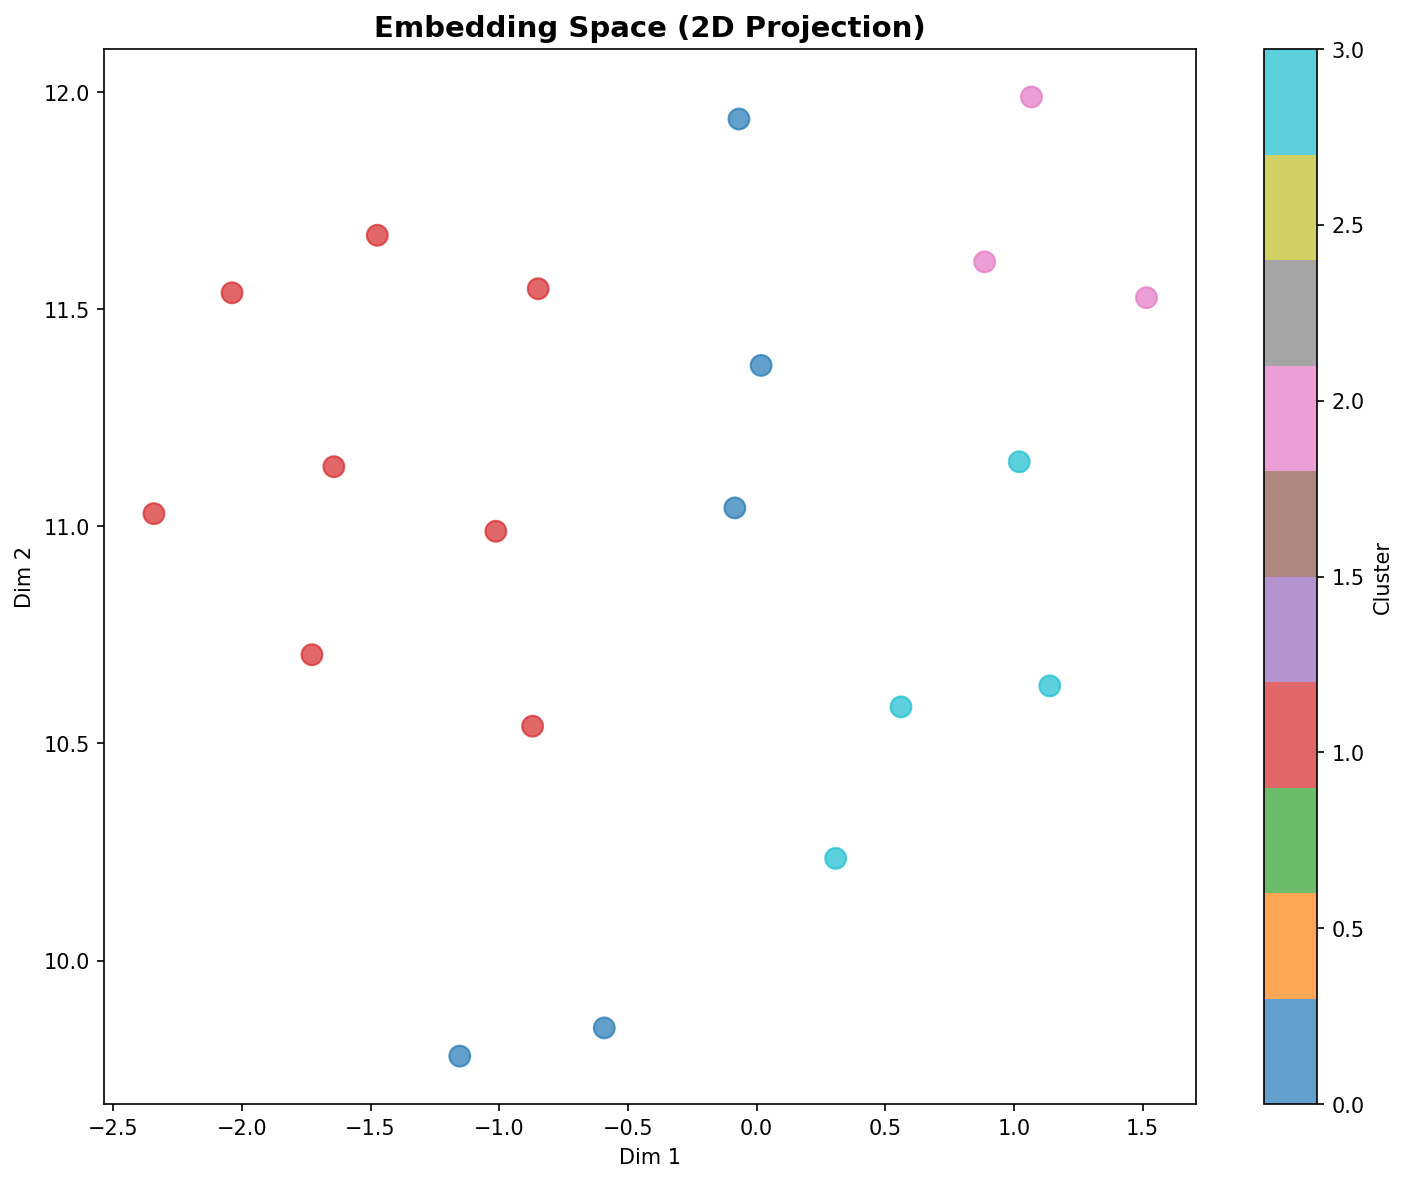
\includegraphics[width=0.8\textwidth]{figures/embedding_space.png}
\caption{t-SNE projection of SentenceBERT embeddings showing modality-based clustering. Image (blue), Text-Translation (orange), Text-QA (green), Audio/Multimodal (red) form distinct clusters.}
\label{fig:embedding-space}
\end{figure}

\section{Feature Extraction Protocol}

\textbf{Decision Rules for Task Type Classification:}
\begin{itemize}
\item Classification: Single-label or multi-label assignment (ImageNet, CIFAR-10)
\item Detection: Spatial localization + classification (COCO, PASCAL VOC)
\item Translation: Sequence-to-sequence transformation across languages (WMT14/16, IWSLT)
\item Question-Answering: Text input + query $\rightarrow$ answer extraction or generation (SQuAD, Natural Questions)
\item Captioning: Image/video $\rightarrow$ natural language description (MS-COCO, Conceptual Captions)
\item ASR: Audio $\rightarrow$ text transcription (LibriSpeech, Common Voice)
\end{itemize}

\textbf{Modality Assignment:}
\begin{itemize}
\item Image: RGB/grayscale pixels (ImageNet, COCO, CelebA)
\item Text: Natural language sequences (WMT, SQuAD, TriviaQA)
\item Audio: Waveforms or spectrograms (LibriSpeech, VGGSound)
\item Multimodal: Requires $\geq 2$ modalities for task completion (MS-COCO captioning, Visual Genome)
\end{itemize}

\textbf{Metric Extraction:}
Extract all reported metrics from benchmark paper abstract and results section. Classify primary metric by prevalence in leaderboard rankings.
